%% 内容梗概

%% git test
%% プリアンブル %%%%%%%%%%%%%%%%%%%%%%%%%%%%%%%%%%%%%%%%%%%%%%%%%%%%%%%%
\documentclass[a4j]{jarticle}

\usepackage{kut-abstract}
%\usepackage[dvips]{graphicx}
\usepackage[dvipdfmx]{graphicx}
\usepackage{utf}
%% 表題 %%%%%%%%%%%%%%%%%%%%%%%%%%%%%%%%%%%%%%%%%%%%%%%%%%%%%%%%%%%%%%%%
%% 注意! 情報学群生の場合は,以下の \ScInfo を有効にすること.
%\ScInfo %% 情報学群生の場合

\Bachelor	%% 卒業研究論文梗概の場合
%\Project	%% プロジェクト研究報告書梗概の場合
%\Seminar	%% 特別研究セミナー課題研究報告書梗概の場合
%\Master	%% 修士学位論文(情報システム工学コース)梗概の場合
%\Doctorate	%% 博士学位論文(情報システム工学コース)梗概の場合
%\English	%% 英語の場合

\Eyears{2017}
\Etitle{English Title}
%\idnumber{}
\Eauthor{YAMASAKI, Naoyuki}
\Eaffiliate{Iwata Lab.}

%% 本文 %%%%%%%%%%%%%%%%%%%%%%%%%%%%%%%%%%%%%%%%%%%%%%%%%%%%%%%%%%%%%%%%

\years{平成29}
\title{LSTM-RNN用アクセラレータ回路の負荷割当法の検討}
\idnumber{1180386}
\author{山 \UTF{FA11} ~~尚 之}
\affiliate{コンピュータ構成学研究室}

%% 本文 %%%%%%%%%%%%%%%%%%%%%%%%%%%%%%%%%%%%%%%%%%%%%%%%%%%%%%%%%%%%%%%%
\begin{document}
\begin{Abstract}

 \section{はじめに}

近年,再帰型ニューラルネットワークRNN(Recurrent Neural Network)が言語処理,音声認識の分野で注目されており,
組込みシステムでリアルタイム翻訳などに用いる場合アクセラレータ回路を使用し,
高速に処理する必要がある.

先行研究として,長期短期記憶LSTM(Long Short-term Memory)を含む微分可能ニューラルコンピュータDNC(Differentiable Neural Computer)
用単一コアの提案\cite{bib:pre-method}がされているが,
単一コアでは処理性能に限界があるためマルチコア化が求められる.

LSTMに代表されるような大規模で複雑なネットワークは今後更に増えると予想され,
これらをマルチコアアクセラレータ回路で動作させると,
1コアあたりの負荷はネットワーク規模に従って大きくなる.
よって,ネットワークに合わせた高効率な負荷割り当て方法を検討することが必要となる.

本研究では,LSTMを一例として取り上げ,マルチコアで動作させる場合の負荷割り当てについて,
今後現れる可能性の高い,
より大きなネットワーク規模の深層ニューラルネットワークDNN(Deep Neural Network)にも対応可能な,
負荷割り当て方法の検討を行う.


 \section{負荷割り当て方法}
単一LSTMアクセラレータ回路の構成は,5段のパイプラインと2つのデータメモリ,
1つのアキュムレータを備えた構造となっている.
各データメモリから演算に必要な対応するデータを取得することで積和演算や積算を行う.
必要に応じて,LUTにあらかじめ登録した活性化関数を参照することで出力を求める.
この一連の流れを繰り返し実行することで,LSTMを行うことが可能である.
このような機能を備えたコアをマルチコアで,
並列処理させる時の負荷割り当てとその負荷割り当てを実現するスケジューリングについて検討を行う.

%負荷割り当ての方法は図\ref{フロー図}に示す3方向の軸に沿った方法が考えられる.
 \begin{figure}[h]
  \centering
  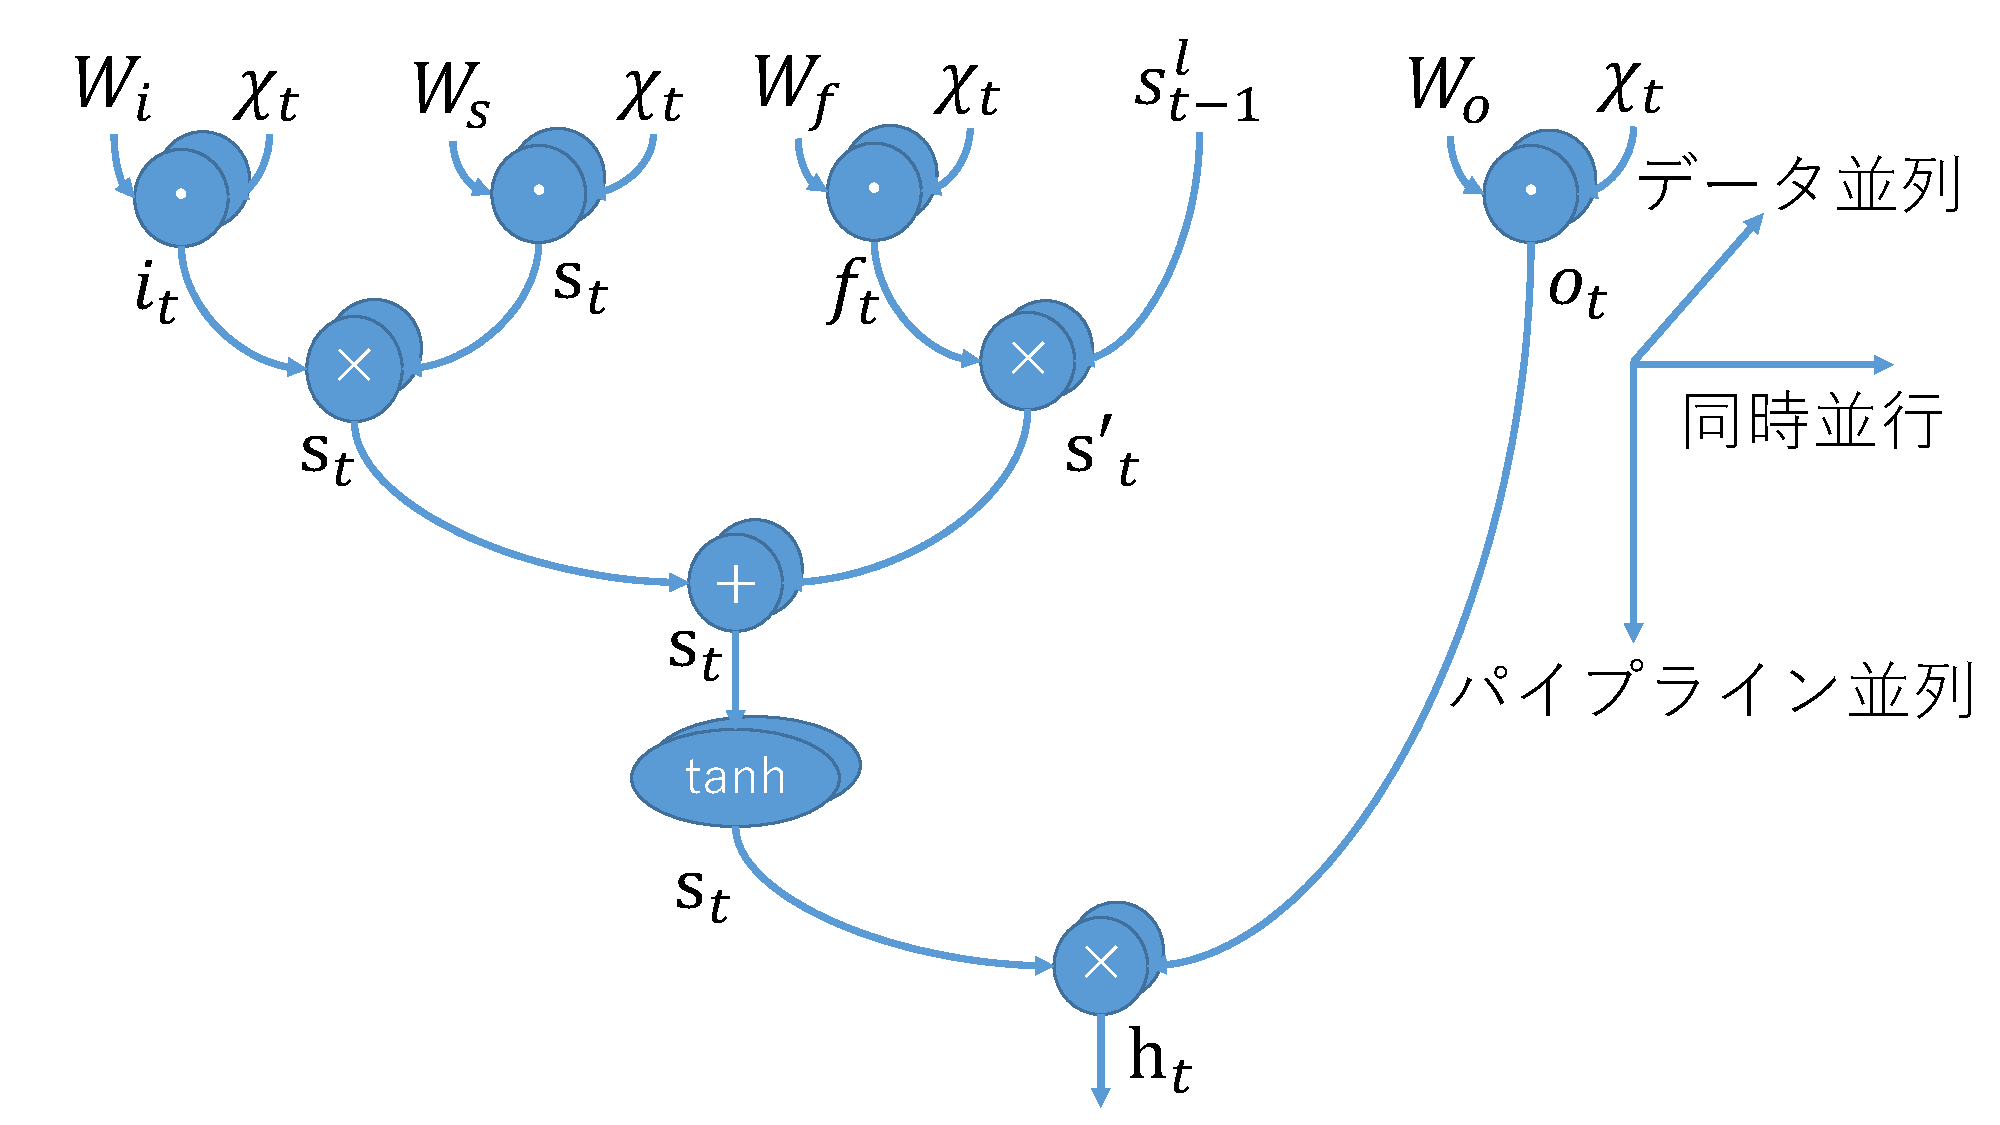
\includegraphics[scale=0.25]{flow.eps}
  \caption{LSTMの計算フロー図}
  \label{フロー図}
 \end{figure}
負荷割り当ての方法は図\ref{フロー図}に示す3方向の軸に沿った方法が考えられる.
同時実行並列方向とパイプライン並列方向の負荷割り当ては,
図\ref{フロー図}の演算命令を左右と上下にそれぞれ分け,
各コアに割り振られた命令を実行する方法である.
データ並列方向の負荷割り当ては全命令を各コアで実行するが,
各演算に必要な行列やベクトルの要素を半分に分ける方法である.
データ並列方向の負荷割り当てではデータの重複を最大限少なくできるが,
演算に必要なデータを半分にして演算を行うため,
図\ref{フロー図}にはない足し合わせの処理が必要となる.

また,データ並列の負荷割り当てを行う際のスケジューリングは,
全ての出力画出揃うまでに次のタイムステップの演算が可能であるというデータ並列の特徴から,
演算命令より入力を受け取るIN命令,結果を出力するOUT命令を優先して行うことで稼働率を高めることが可能である.

 \section{性能の見積もり}
 コア数32,中間層のニューロン数256,入力数128とした場合の
 性能について見積もりを行った.
 各割り当て方法の実行時間と回路面積を
 1回の演算処理にかかる時間,1回の通信にかかる時間,
 1要素のデータを保存するためのメモリ領域をそれぞれ1として概算し比較を行った.
 結果として,データ並列方向に負荷割り当てを行った場合,
 二番目に性能の良い同時実行並列方向の割り当てに比べ,
 7.2\%低負荷での実行が可能であるという見積もり結果が得られた.

次に,最も性能の高い結果が得られたデータ並列方向の負荷割り当てについて,
NOP命令の実行回数を調べ
稼働率を式(\ref{ラベル})により求める.
\begin{equation}
  稼働率 = \frac{実行命令数}{実行命令数+NOP命令実行数}
  \label{ラベル}
\end{equation}

LSTMを実行した場合,
1タイムステップで1コアあたり実行されるNOP命令は330回であり,稼働率は97.4\%であった.
また,コア数を固定し中間層のニューロン数を増加させると,
稼働率が上昇することが分かった.
これはニューロン数を増加させた場合,通信命令より演算命令の増加率が高いため,
通信網が占有されている時に演算命令を代行できる確率が増えるからであると考えられる.

 \section{まとめ}
負荷の割り当て方法として,
データ並列方向の負荷割り当てが3つの割り当て方法の中で,
実行時間,回路面積の観点から最も性能が高くなるという見積もり結果が得られた.
また,稼働率がネットワーク規模の大きさに伴い上昇することから,
より複雑で演算回数の多いネットワーク構成のDNNであっても,
高稼働率での実行が可能であるといえる.
今後,この見積もりをもとに実装を行い,実際の性能評価を行う.


%% 参考文献 %%%%%%%%%%%%%%%%%%%%%%%%%%%%%%%%%%%%%%%%%%%%%%%%%%%%%%%%%%%%
\begin{thebibliography}{99}
 \bibitem{bib:pre-method} Akane Saito, Yuki Umezaki, and Makoto Iwata,
  ``Hardware Accelerator for Differentiable Neural Computer and Its FPGA Implementation,
  ''PDPTA'17, pp.232-238, July 2017.
\end{thebibliography}

\end{Abstract}
\end{document}
